\documentclass[a4paper]{ctexart}
\usepackage{geometry}
\usepackage{hyperref}
\geometry{left=2cm,right=2cm,top=2.5cm,bottom=2.5cm}
\setCJKmainfont[BoldFont={SimHei},ItalicFont={KaiTi}] {SimSun}

\author{严春伟}
\title{WBIA报告}
\begin{document}
    \maketitle
%---content here----
我做的第 2 题,用的是 SST 算法。 \\
代码寄存在 github 上,开发语言为 Python2.7   
    \begin{description}
        \item [Git] \href{https://github.com/superjom/TDA.git}{https://github.com/superjom/TDA.git}
        \item [Pos] \href{https://github.com/superjom/TDA/tree/master/pySST}{https://github.com/superjom/TDA/tree/master/pySST}
    \end{description}

\section{实现内容}
本实验实现了 SST 算法,通过扫描一个网页集在内存中维护一个风格树,然后通过统计,
将原来网页中的相应正文以及噪音节点通过改变其背景颜色标识出来。
\par 在后期测试期间,本实验自行爬取了 MSN.com 网站 207 个网页进行了处理。算法实现结果主要以直接标注 html 代码的方式返回,可以通过浏览器查看标注后的网页。测试结果表明原生的 SST 算法非常关注新鲜多变的内容作为正文,因此,如果把博客中的回复内容作为正文的话,那么 SST 效果可以,但是如果评论作为噪音的话,SST 效果并不会很好。 \\
\section{程序构成}
自己实现的程序主要有三部分: 
\begin{enumerate}
    \item 爬虫(reptile)\\
    单线程的 python 实现的简单爬虫,在爬取的时候,为了防止频繁访问被服务器屏蔽,采用 5-20s 的随机间隔时间进行爬取。爬取的目标网站是 news.MSN.com,主要考虑的是: 
    \begin{itemize}  
        \item 标签相对规整,降低 html 解析错误 
        \item utf-8 编码,减少 gbk 转码发生的乱码 
    \end{itemize}
  \item SST 算法(Site Style Tree) \\
    基本上是论文中算法的实现,感觉算法的复杂度比较高,实际应用中,发现SST算法的一个问题(至少论文里面的)——忽略非叶子节点的feature内容。 这个会在后面"算法改进"章节讲。
  \item 数据可视 \\
    之前跟研二的学长讨论过,应该是要用人工标注的方式通过召回率等指标来验证具体的
效果,但由于时间关系,退而求其次。 \\
    为了方便测试,实现了一个简单的数据可视化模块,有两个功能: 
    \begin{enumerate}
        \item 将内存中的 SST 树以 pdf 的格式输出为树形图\\
        采用 graphviz 工具,对于小数据效果非常出色(MSN 的网页支持 3 个,<2000 个节点),但是对于大点的数据失效(pdf 展开面积过大) 
        \item 直接对原有的 html节点用背景色标注\\
        算法会对Html 源文件扫描两次,第一次建成 SST 树,第二次根据 SST 树标注 html中的节点,将识别出的噪音节点背景色改为灰色,对识别出的正文部分背景色标注为蓝色 
    \end{enumerate}
\end{enumerate}

\section{算法及程序描述}
\subsection{爬虫(Reptile)}
路径:pySST/reptile/ \\
由三个类组成: \\
\begin{tabular}[t]{ll}
    Reptile & 爬虫主程序 \\
    Urlist & 判断 URL 是否重复访问 \\
    SourceParser & 解析 html,抽取出 URL,并且判断筛选出合乎要求的 URL 
\end{tabular}

\subsection[t]{SST}
路径:pySST/sst \\ 
\textbf{Styletree.py}  定义了一些风格树相关的数据结构: \\
\begin{tabular}{ll}
    ElementNode& 普通标签 \\
    DataNode& 内容标签,包含若干 features,每个ElementNode默认有一个 DataNode\\
    StyleNode&  风格节点 \\
    StyleTree& 风格树结构,包含一个body的ElementNode
\end{tabular}\\
\textbf{Sourceparser.py} 解析 html,调用 styletree 建立 SST \\
\textbf{dic} 字典模块,在 SST 的 feature 熵计算中,用 md5 为此网页集合每个feature建立了一个字典项,在全局维护了一个字典,为每一个feature一个ID以压缩存储空间。
\par 每个DataNode会有一个局部字典,以记录非重复的feature\quad ID\\
\begin{tabular}{ll}
    dic.py &字典基类\\
    nodedatas.py &为每一个节点建立了一个局部的字典,便于统计 \\
\end{tabular}
\subsection{SST结构演示}
    %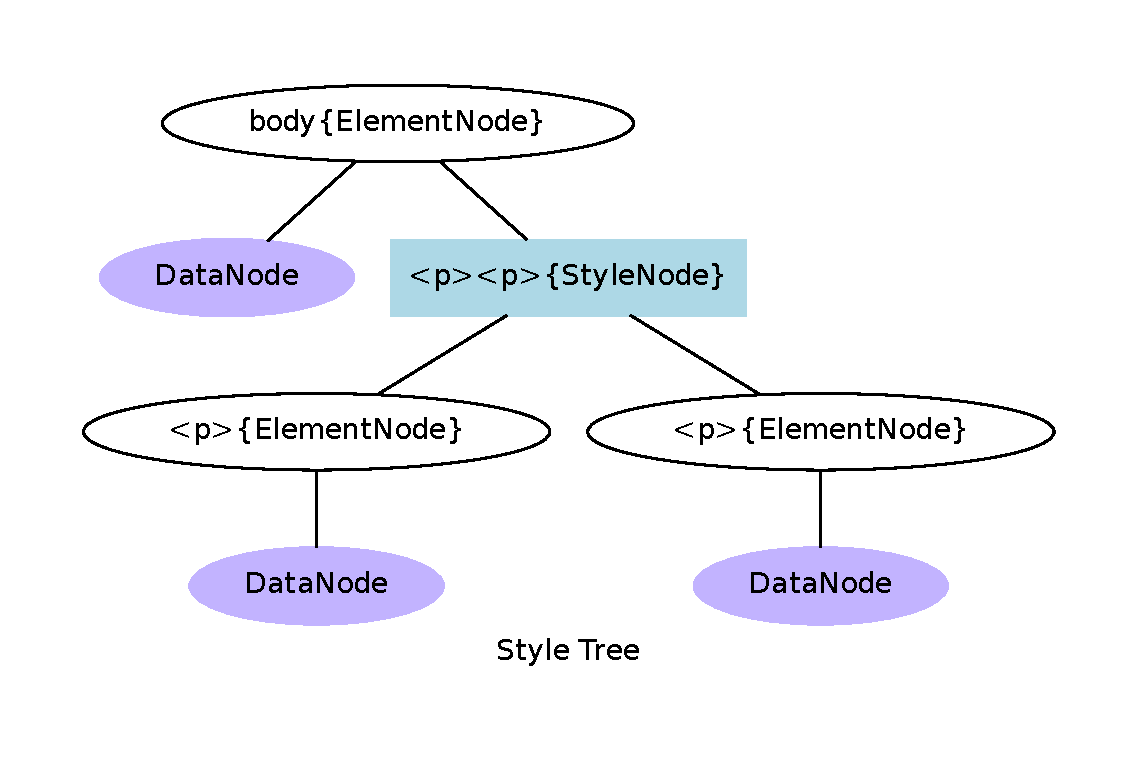
\includegraphics[height=6cm]{../dot/data_structure_demo.pdf}
    \begin{center} 
    \includegraphics[height=6cm]{../dot/ignore_data_of_node.pdf}\\
    \textbf{figure 1}
    \end{center}
\par 总之,一个 ElementNode 默认有一个 DataNode(记录其直接拥有的内容features,DataNode数据可以为空),可以有多个 StyleNode;  一个 StyleNode可以有多个 ElementNode 
\par 初始化:为 body 标签建立一个 ElementNode,将此 ElementNode 及 HTML 树中的 body 节点压入栈,此后循环迭代,pop 出节点对,以深度优先方式便利 HTML 树,同时建立 SST。 

\subsection{数据可视化}
\begin{tabular}[t]{ll}
    doter.py    &   将 SST 输出为 dot 文件,用 graphviz 画出树形图 \\
    temdec      &   模板标注,采用 css 将正文标注为蓝色底红框,噪音标注为灰色底黄框\\
                &以色块方式直接标注实验数据中的网页,并输出为 HTML 文件 \\
    dotter.py      &   将 SST 转化为树形图的 .dot文件\\
                    &然后利用graphviz工具转化为pdf 文件,方便小规模数据的测试和调试 \\
\end{tabular}

\section{算法改进}
\par 作者论文中介绍的,每个Element权重计算的公式
{\zihao{5}{
$$
CompImp_{former}(E) = (1-r')NodeImp(E) + r' \sum_{i=1}^{l}{p_iCompImp(s_i)}
$$}
$$
CompImp(S_i) = \frac{
        \sum_{j=1}^{k}{CompImp(E_j)}
    } {k}
$$}
\par 基于公式及论文可以得到,对于每个非leaf node的Element的权重涉及到:\\
\begin{tabular}[t]{ll}
    $NodeImp(E)$ &  拥有的风格样式(StyleNodes)的熵\\
    $CompImp(S_i)$ & 子孙节点权重的传递\\
\end{tabular}
\\
整个计算过程\textbf{\color{red}忽略了叶子节点拥有的feature}\\
\fbox{例如}\\
\includegraphics[height=2cm]{ignore_data_of_node.png}\\
参照上面的\textbf{figure 1},<div\#content>不是叶子节点,其包含的文本feature(构成了DataNode)被漠视\\
实验中,我们将内容feature的重要性与其原来的重要性以一定比例中和(如果Element有feature)
{\zihao{5}{
$$
CompImp_{final}(E) = (1 - k)CompImp_{former}(E) + k*DataNode(E) 
$$
$$
k = \frac{DataNode(E)}{
        CompImp_{former}(E) + DataNode(E)
    }
$$
}}

\\
\\
\section{测试及总结}
\begin{center}
    \fbox{from}\\
    \includegraphics[height=6cm]{html_source_1.png}\\
    \fbox{to}\\
    \includegraphics[height=6cm]{html_source_2.png}
\end{center}
\subsection{不足}
本实验在很多方面还有许多需要改进:
\begin{enumerate}
    \item 解析HTML的库,pyquery过于单薄,应该采用firefox引擎或者webkit,性能和效果都更能有保证 
    \item 测试结果,还需要以更加严谨和量化的方式呈现
    \item 程序模块的架构应该更加合理一点,融入更多OOP的思想,优化各个模块间的关系
\end{enumerate}
\subsection{收获}
\par 大四的时候接触SST,非常推崇它的理念。但是现在具体实现了之后,觉得毕竟是十年前的算法,在现在这样的环境还是有很多不足的。 比如现在的网页标签更多,标签的组合也更加异变,这让基于标签组合(sytle node)的SST过于敏感,伴随着过多的style node的分割,ssytle node下的elements也支离破碎,似乎难以有全局的考量。
\par 这让我认识到,要了解一个思想,最切实的是要去实现出来,客观分析。 理论和现实需要用实践去统一。
\par 实验中走了一些弯路,实验的过程也比较漫长,更让我认识到,人的精力和时间总是有限的。如何用有限的时间,集中精力去做好有限的事情。回到学术研究上,还是应该抓住一个点,持之以恒。这个是我缺少的,也是需要立即去做的。

\end{document}


